\documentclass[a4,12pt]{scrartcl}
\usepackage[margin=3cm]{geometry}
\usepackage[francais]{babel}
\usepackage[utf8]{inputenc}
\usepackage{amsmath}
\usepackage{graphicx}
\usepackage{subcaption}
\usepackage[colorinlistoftodos]{todonotes}
\usepackage{tabularx}
\usepackage{colortbl}
\usepackage{hyperref}
\usepackage{float}

\title{Réalité Virtuelle}
\subtitle{Étude documentaire}

\author{Corentin Smith}
\date{\today}

\begin{document}
\maketitle

\newpage
\tableofcontents

\newpage
\section{Introduction}

\section{Définitions et histoire}

\subsection{Naissance}

Le premier système pouvant s'apparenter à de la réalité virtuelle dans l'acception moderne du terme est sans doute le Sensorama de Morton Heilig \cite{Sensorama}. Sorti en 1962, il s'agit d'une station composée d'un écran, d'un diffuseur d'odeurs, de son stéréo, d'un siège vibrant, et d'un ventilateur destiné à simuler le vent dans les cheveux de l'utilisateur. Jusqu'à 4 stations peuvent être connectées afin d'avoir une expérience partagée.

\begin{figure}[H]
	\centering
	\begin{subfigure}{.4\textwidth}
	  \centering
	  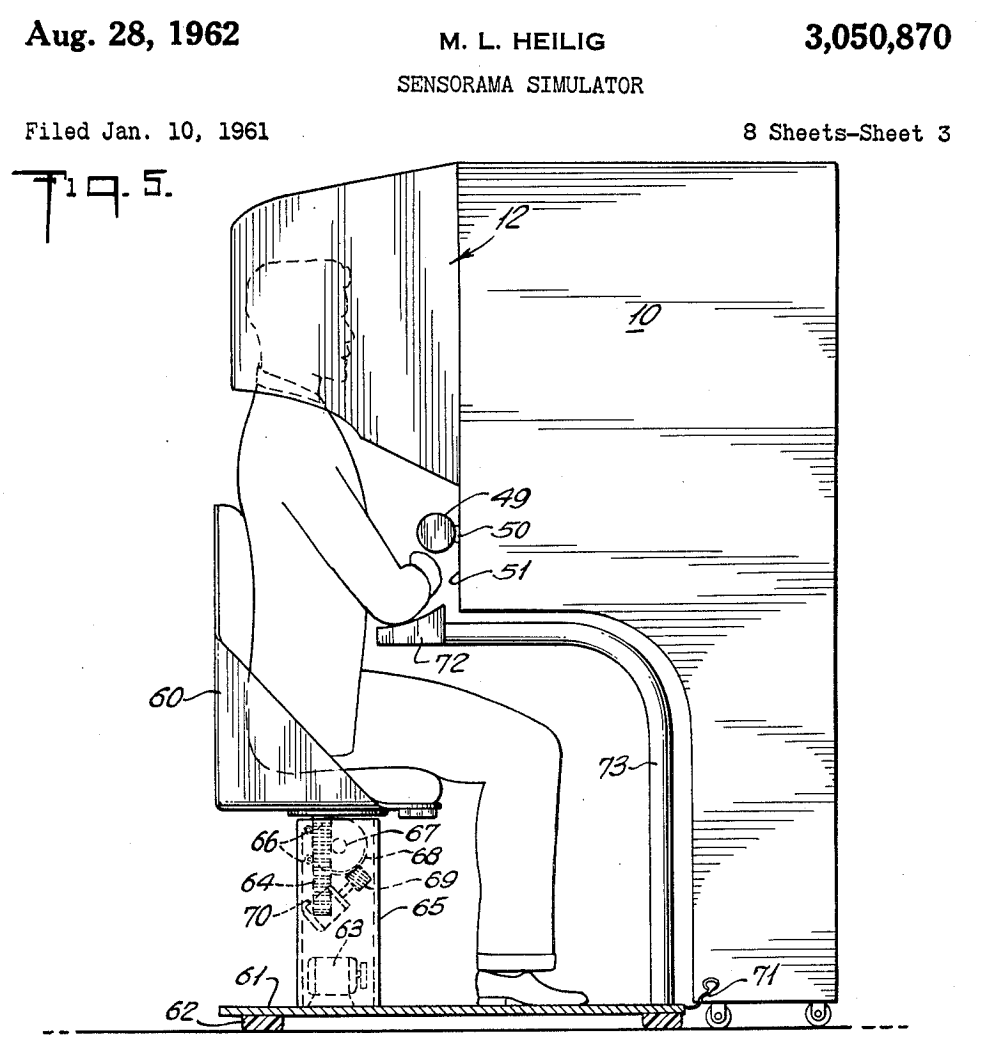
\includegraphics[width=\linewidth]{sensorama-patent}
	\end{subfigure}
	~
	\begin{subfigure}{.4\textwidth}
	  \centering
	  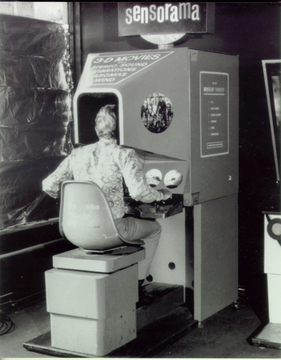
\includegraphics[width=0.8\linewidth]{sensorama}
	\end{subfigure}

 	\caption{Sensorama, Morton Heilig}
\end{figure}



\begin{figure}[H]
	\centering
	\begin{subfigure}{.4\textwidth}
	  \centering
	  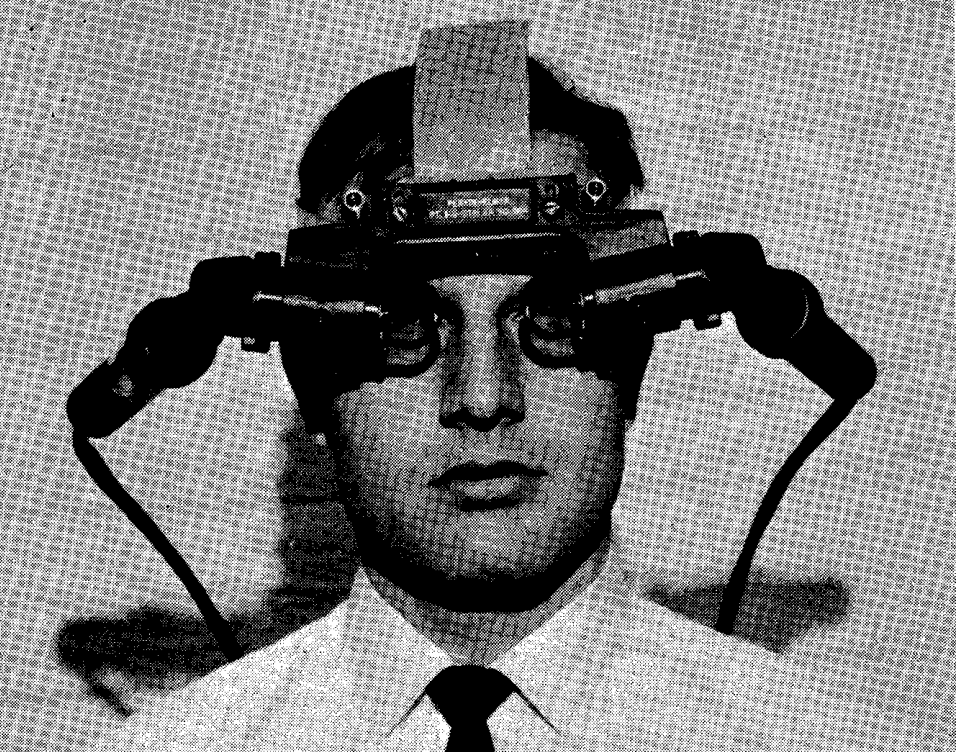
\includegraphics[width=\linewidth]{sutherland-1}
	\end{subfigure}
	~
	\begin{subfigure}{.4\textwidth}
	  \centering
	  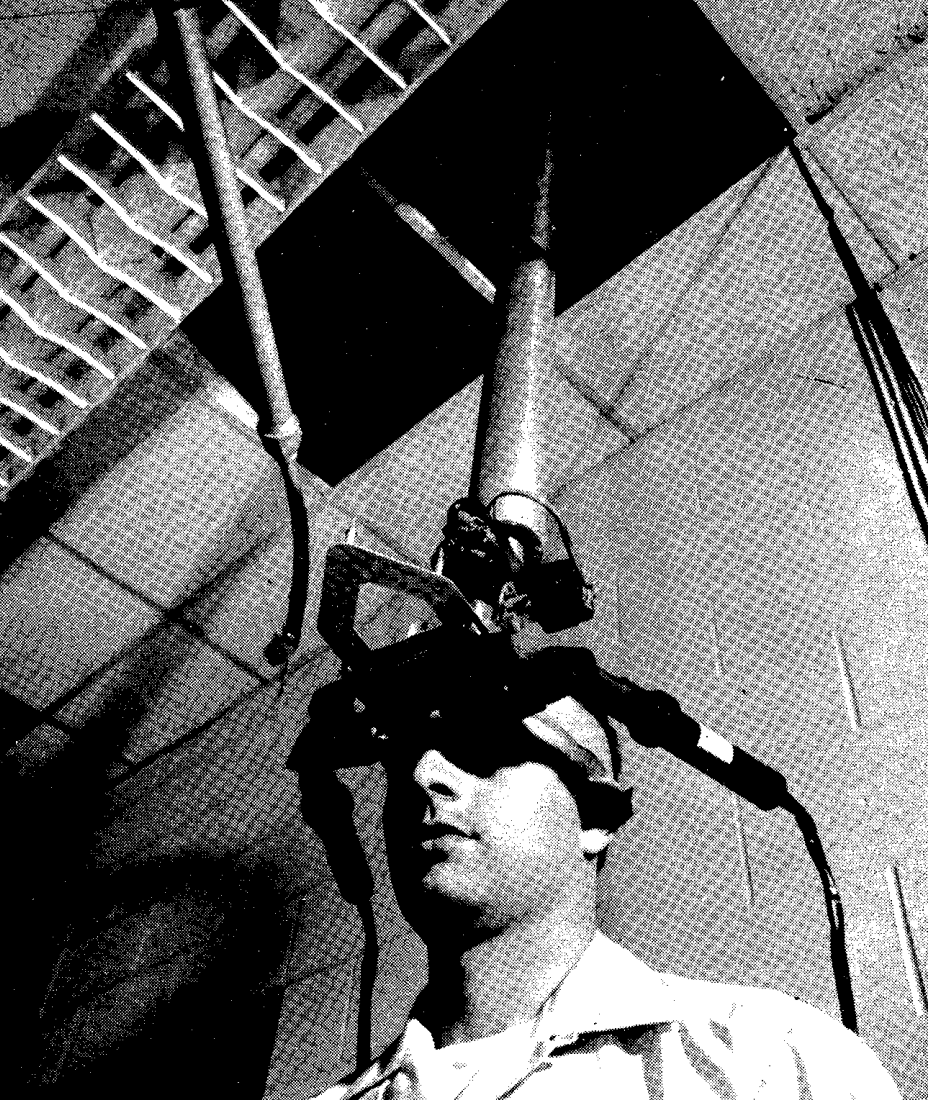
\includegraphics[width=0.8\linewidth]{sutherland-2}
	\end{subfigure}
 	\caption{Sutherland \cite{Sutherland68}}
\end{figure}

\subsection{Années 80}

\begin{figure}[H]
	\centering
	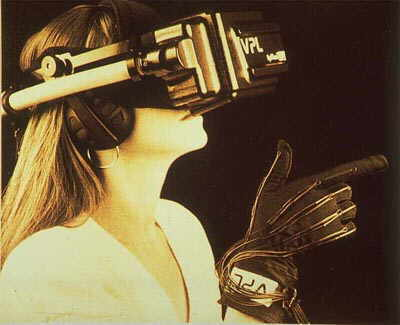
\includegraphics[width=0.6\linewidth]{vpl-hmd}
	\caption{VPL Research}
\end{figure}

Dans les années 80, la recherche s'intensifie, poussée notamment par des investissement de la NASA et du département américain de la défense [citation needed]

\subsection{Années 90}

\begin{figure}[H]
	\centering
	\begin{subfigure}{.4\textwidth}
	  \centering
	  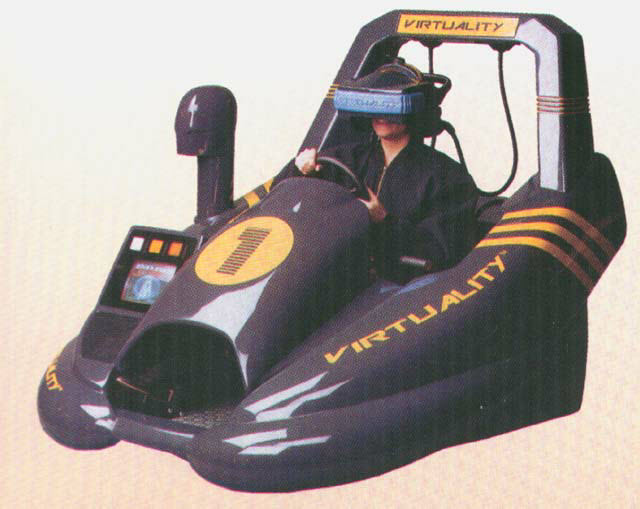
\includegraphics[width=\linewidth]{virtuality}
	  \caption{\emph{VR Pod} de Virtuality (1991)}
	\end{subfigure}
	~
	\begin{subfigure}{.4\textwidth}
	  \centering
	  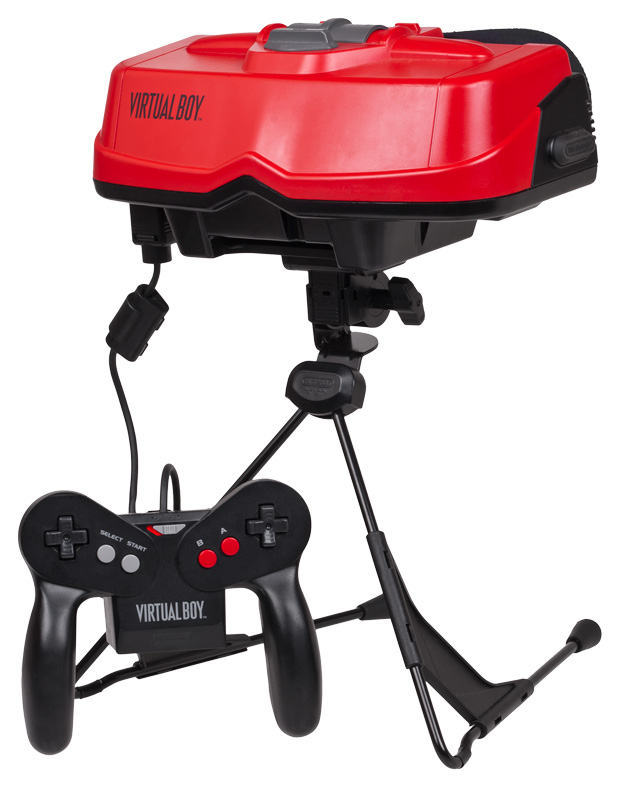
\includegraphics[width=0.8\linewidth]{virtualboy}
	  \caption{Nintendo Virtual Boy (1995)}
	\end{subfigure}
 	\caption{Systèmes de réalité virtuelle des années 90}
\end{figure}

Les années 90 sont l'âge d'or de la réalité virtuelle grand public.


En 1991, \emph{Virtuality} lance le premier système de réalité virtuelle grand public. Il comportait des lunettes et des gants à exosquelette, ce qui en fait la première expérience immersive de réalité virtuelle. Vendu pour environ \$60 000 l'unité, il est destiné principalement au salles d'arcades.

\subsection{Notion de présence}


\section{État de la technologie}


\subsection{Systèmes de vision}

Les systèmes de vision pour la réalité virtuelle actuels se présentent à peu près tous sous la forme : un ou deux écrans d’une dizaine de centimètres de diagonale sont placés sur une sorte de masque, couvrant les yeux de l’utilisateur. La position et/ou l’orientation de la tête sont mesurées par des capteurs internes ou externes, et l’utilisateur peut ainsi s’orienter dans le monde virtuel.\\

Michael Abrash liste dans sa conférence \cite{Abrash14} les différents paramètres les plus importants à prendre en compte dans les systèmes de vision pour arriver à une sensation de présence. Regardons ici les plus importants.

\subsubsection{Champ visuel}

Le champ visuel est défini comme l'ouverture angulaire dans laquelle l'utilisateur peut voir la scène virtuelle. Selon Abrash, la présence commence aux environs de 80 degrés d'ouverture et s'améliore significativement vers 110 degrés, ce qui correspond plus ou moins à la partie vision binoculaire du champ de vision humain. La plupart des appareils actuels ne dépassent pas 110 degrés de champ de vision.

\subsubsection{Résolution}

La résolution est un aspect évidemment très important d'une expérience de réalité virtuelle ; l'écran étant en général placé très proches des yeux de l'utilisateur, la résolution angulaire est assez faible en comparaison à un écran classique d'ordinateur ou de téléphone.

La résolution angulaire d'un \oe{}uil nu est de l'ordre d'une arcminute, ou $0,016$ degrés. Pour arriver à cette résolution angulaire avec un champ de vision de 110 degrés, il faudrait une résolution d'environ $6600 \times 6600$ (dans un format d'environ 4cm $\times$ 4cm si on place l'écran à une distance de 3cm de l'\oe{}uil, ce qui donne une densité de 4200 pixels par pouce).

On est donc encore loin d'être à ces niveaux de densité puisque les écrans les plus fins actuels arrivent tout juste à 500 pixels par pouce ; ce qui correspond au dernier prototype d'Oculus Rift, annoncé cette année au CES, qui est supposé avoir un écran de 2560 $\times$ 1440.

\subsubsection{Faible persistence}

La persistence est la durée pendant laquelle un pixel de l'écran reste allumé. Ce n'est pas un paramètre très important pour la plupart des écrans, mais dans le cas de la réalité virtuelle l'écran est placé très près des yeux, ce qui augmente le mouvement relatif de ces derniers par rapport aux pixels.

\begin{figure}[H]
	\centering
	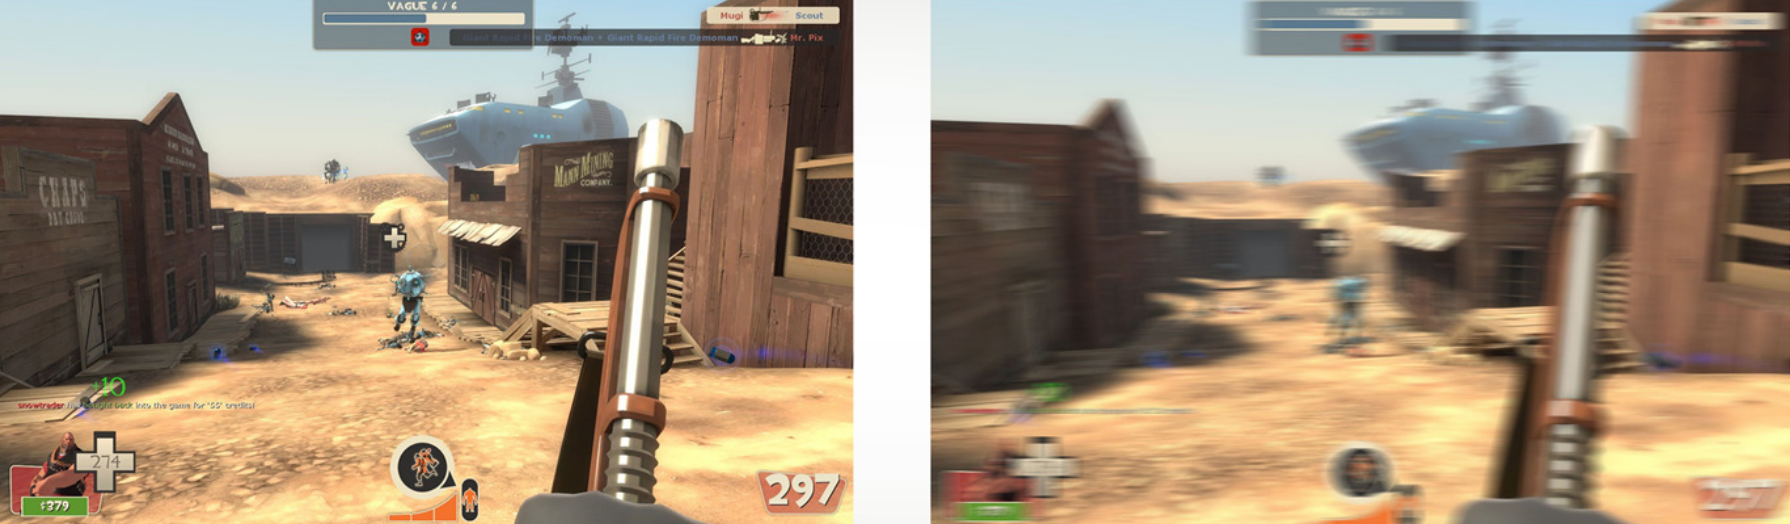
\includegraphics[width=\linewidth]{persistence}
	\caption{Simulation de l'effet de la persistence de l'image sur l'écran.}
\end{figure}

Une persistence de l'ordre de 3ms semble être suffisamment basse pour les systèmes actuels \cite{Abrash14}.

\subsubsection{Haut taux de rafraichissement}

Le fait de diminuer la persistence des pixels pose un problème visuel : l'image semble clignoter puisqu'elle est noire la plupart du temps. La persistence rétinienne ne suffit pas à compenser cet effet lorsque la fréquence de rafraichissement de l'image est trop faible.

En effet, à 60Hz, on a une image toutes les 16ms environ. Si chaque pixel ne reste allumé que 3ms, on a un “trou” de 13ms pour chaque image où l’écran n’affiche rien, ce qui est visible par l’utilisateur. Une fréquence de l’ordre de 95Hz semble être suffisante pour une expérience ne causant pas de nausées.


\subsubsection{Optique}

La conception du système optique d’un casque de réalité virtuelle est importante pour l’immersion. Un système idéal devrait permettre de régler simultanément : 
\begin{itemize}
	\item la distance focale
	\item la distance de visionnement
	\item la taille perçue de l’image
	\item la distortion
	\item les aberrations chromatiques
\end{itemize}

Cependant un système de cette nature devrait utiliser plusieurs lentilles en conjonction, et atteindrait des tailles et un poids qui ne sont pas en accord avec un dispositif pouvant tenir sur le visage de l’utilisateur (voir Figure~\ref{ideal-lens}).

\begin{figure}[H]
	\centering
	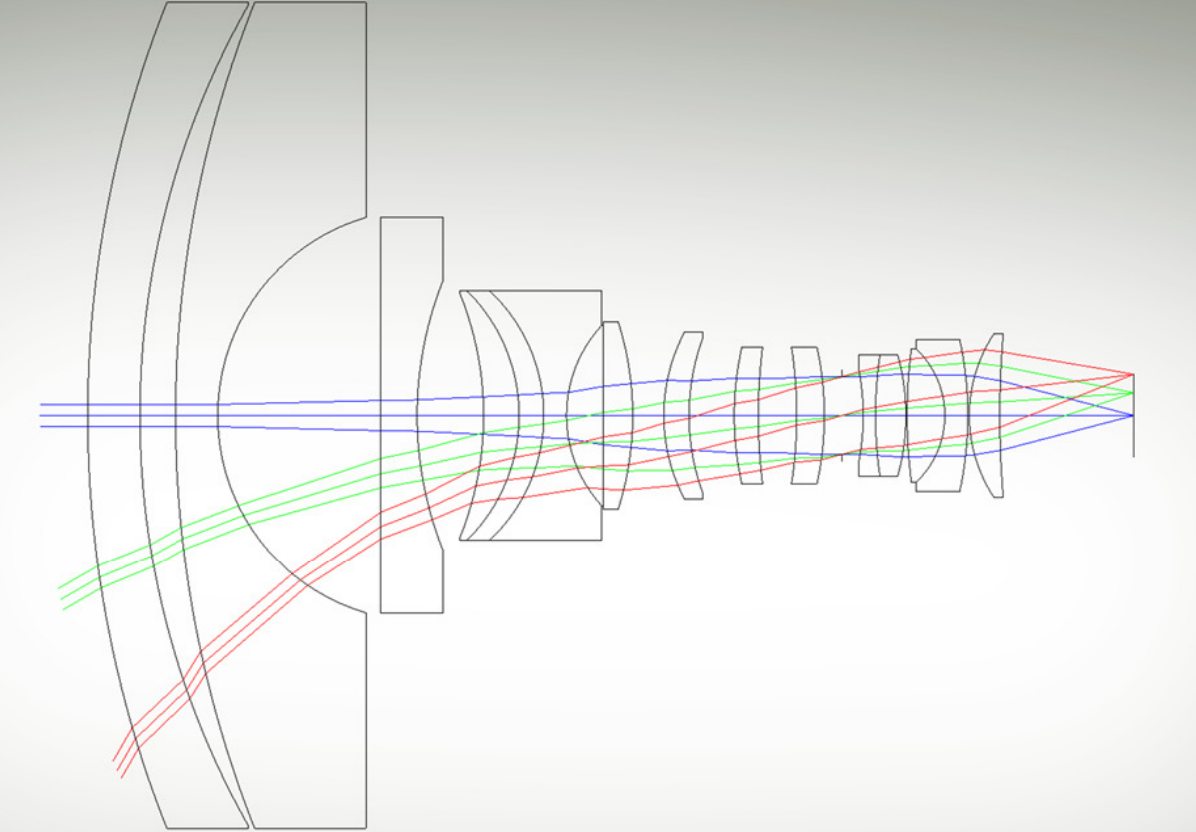
\includegraphics[width=0.6\linewidth]{lens}
	\caption{Système optique idéal (Valve) -- les plus grandes lentilles font plus de 30cm de diamètre}
	\label{ideal-lens}
\end{figure}

Un compromis est donc nécessaire dans la réalisation pratique, comme on peut le voir avec les lentilles de l’Oculus Rift, qui utilisent une forme carrée peu conventionnelle. Certains des défauts évoqués précédemment peuvent également être corrigés au niveau du logiciel, comme la distortion et l’aberration chromatique.

\begin{figure}[H]
	\centering
	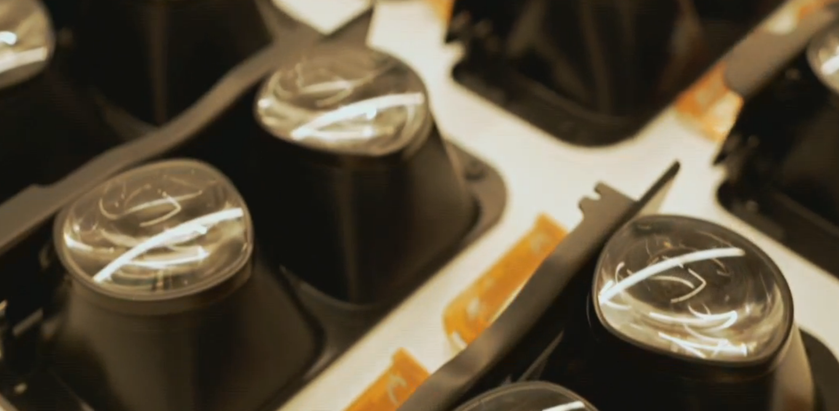
\includegraphics[width=0.7\linewidth]{crescent-bay-lens}
	\caption{Lentilles du dernier prototype de l’Oculus Rift}
\end{figure}

\subsubsection{Calibration optique}

Il ne suffit pas d’avoir de bonnes lentilles pour que les problèmes liés à l’optique soient réglés ; il faut également que le dispositif puisse s’adapter à l’utilisateur de manière très précise. Nous sommes extrêmement sensibles aux moindres erreurs de représentation du monde virtuel. Un exemple paramètre à régler individuellement est celui de la distance inter pupillaire, qui donne une information de taille aux objets vus dans la simulation.

\subsubsection{Tracking robuste}

Afin de retranscrire fidèlement les mouvements de l’utilisateur dans l’espace virtuel, une solution de tracking de la position et de l’orientation de la tête est nécessaire. Ce positionnement doit se faire de manière absolue, c’est-à-dire éviter la dérive. Une précision de l’ordre du millimètre dans les trois dimensions est requise.

\subsubsection{Temps de latence}

La perception du temps de latence est critique pour arriver à une sensation de présence.

Michael Abrash \cite{Abrash12} et John Carmack \cite{Carmack13} postulent qu’une latence \emph{“motion to photon”} de 20ms est la durée maximum pour ne pas être perceptible. Ceci pose problème car les technologies LCD ne sont pas conçues pour donner une faible latence.

\todo{étoffer}


\subsection{Systèmes audio binauraux}

Le champ de l’audio pour la réalité virtuelle est en train de prendre de l’ampleur, mais il n’a pas toujours été dans les priorités des constructeurs de matériel de réalité virtuelle.

\begin{figure}[H]
	\centering
	\begin{subfigure}{.3\linewidth}
	  \centering
	  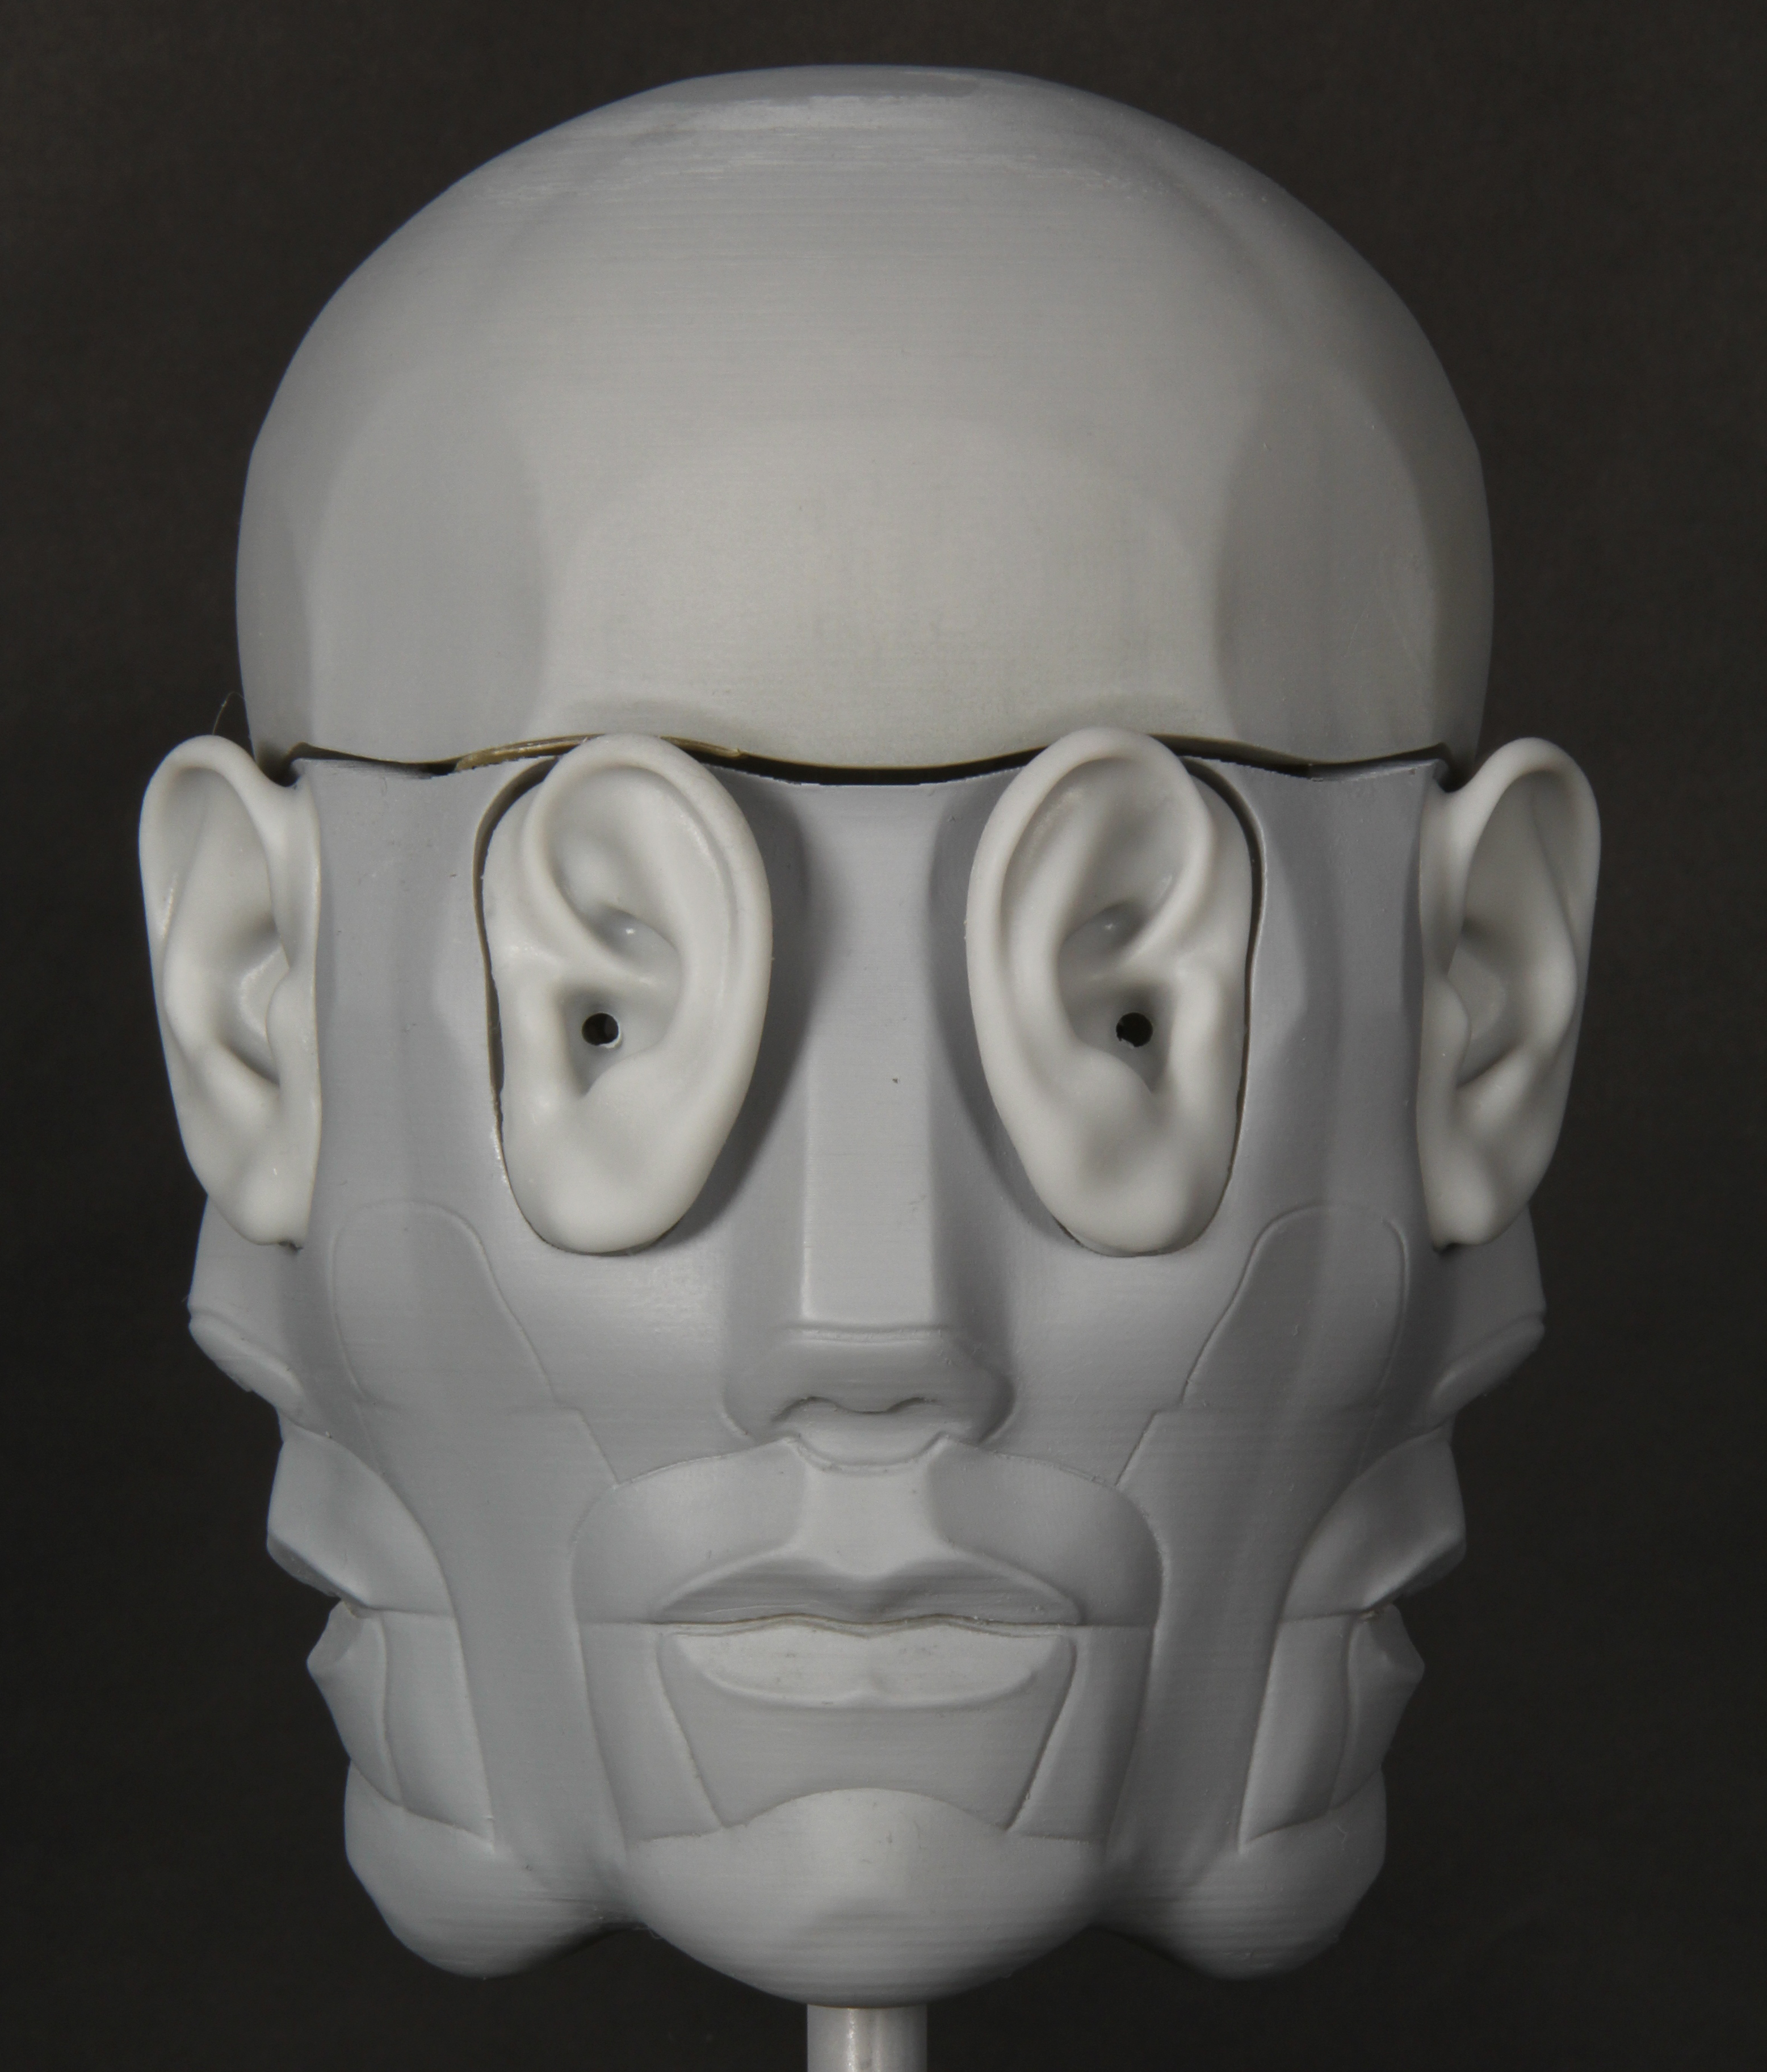
\includegraphics[width=\linewidth]{binaural-3d-microphone-head}
	\end{subfigure}
	~
	\begin{subfigure}{.3\linewidth}
	  \centering
	  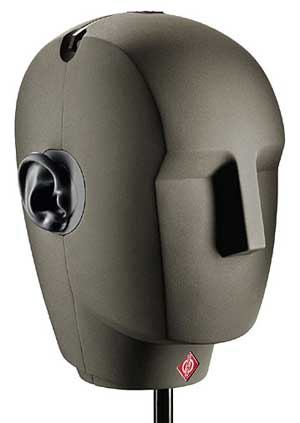
\includegraphics[width=0.8\linewidth]{ku-100}
	\end{subfigure}
 	~
	\begin{subfigure}{.3\linewidth}
	  \centering
	  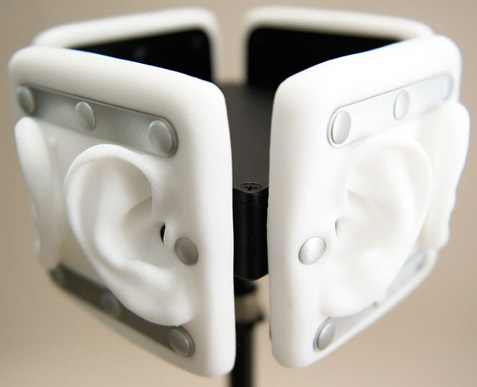
\includegraphics[width=\linewidth]{freespace-omni}
	\end{subfigure}
 	\caption{Différents micros pour enregistrement binaural}
\end{figure}

\subsubsection{Principe de fonctionnement}
\subsubsection{Problématiques}
\subsubsection{Encore un truc}

\subsection{Systèmes maîtres/esclaves}

\subsubsection{Origine}

CEA

\subsubsection{Paramètres clés}

\subsubsection{Nouveaux entrants}

Dexta Robotics




\section{Développements récents et futurs}

\subsection{Oculus}

\subsection{Grand public enfin possible ?}



\newpage
\bibliography{bibliography}
\bibliographystyle{plain}


\end{document}





